\chapter{La recommendation}

\section{Introduzione alla recommendation}

Come fa \textit{Spotify} a sapere quale canzone l'utente vorrebbe ascoltare? E come fa \textit{Netflix} a suggerire la prossima serie da guardare? Questo è possibile grazie ad un sistema di \textit{recommendation} che, utilizzando tecniche di \textit{machine learning}, analizza cosa piace all'utente e gli propone contenuti su misura. 

Solitamente si utilizzano due tipi principali di raccomandazioni:

\begin{itemize}
    \item per la \textit{home page}: sono raccomandazioni personalizzate per un utente in base ai suoi interessi. Ogni utente vede articoli diversi
    \item su articoli correlati: sono raccomandazioni simili a un articolo specifico. Per esempio in \textit{Google Play}, gli utenti che visualizzano la pagina di un'app di matematica potrebbero vedere anche un riquadro con app correlate, come altre app di matematica o di scienze
\end{itemize}

Questo sistema aiuta gli utenti a scoprire contenuti interessanti all'interno di un'enorme quantità di dati. Per esempio su \textit{YouTube} ci sono miliardi di video, con nuovi contenuti che vengono aggiunti ogni giorno. Come può un utente trovare qualcosa di nuovo che valga la pena guardare o provare? La ricerca manuale è un'opzione. Tuttavia, un motore di \textit{recommendation} è in grado di suggerire contenuti che magari l'utente non avrebbe mai pensato di cercare da solo. Basti sapere che, secondo quanto dice la pagina di \href{https://developers.google.com/machine-learning/recommendation/overview}{Google Developers - Recommendation Systems Overview}:

\begin{itemize}
    \item il 40\% delle app installate dal \textit{Google Play} derivano da raccomandazioni
    \item il 60\% del tempo di visualizzazione su \textit{YouTube} proviene dalle raccomandazioni
\end{itemize}

Ci sono alcuni termini da introdurre:

\begin{itemize}
    \item \textit{sistema}: è il motore di \textit{recommendation} che, dato in input una \textit{query}, restituisce una lista ordinata di \textit{item} che si stima siano rilevanti o interessanti per l'utente in quel contesto
    \item \textit{item}: sono gli elementi/entità raccomandate dal sistema. Su \textit{Spotify} sono le canzoni, su \textit{Amazon} sono i prodotti, su \textit{Instagram} sono i \textit{post}.
    \item \textit{feedback}: sono le interazioni che legano l'utente agli \textit{item}, le informazioni pregresse con cui si costruisce il sistema. Possono essere espliciti (e.g. valutazioni, \textit{like}, etc.) o impliciti (e.g. numero visualizzazioni, acquistato o meno, etc.)
    \item \textit{query}: è una richiesta di raccomandazione, ovvero una domanda posta al sistema per ottenere suggerimenti personalizzati. Le \textit{query} possono essere una combinazione di informazioni dell'utente (e.g. ID, elementi con i quali ha interagito in passato, etc.) e contesto aggiuntivo (e.g. ora del giorno, per quanto tempo ha osservato quel prodotto o quell'episodio, etc.)
\end{itemize}

Per la creazione del sistema i passaggi tipici sono:

\begin{enumerate}
    \item collezione dei dati: raccolta dei feedback tra utenti e \textit{item} (e.g. valutazioni, click, acquisti, etc.)
    \item preprocessing dei dati: pulizia e trasformazione dei dati raccolti per renderli utilizzabili dal sistema di \textit{recommendation}
    \item creazione dei modello: addestramento di una serie di modelli di \textit{machine learning} sui dati pre-elaborati per apprendere le relazioni tra utenti e \textit{item}
\end{enumerate}

Una volta che i modelli sono addestrati, il sistema di \textit{recommendation} può essere utilizzato per generare raccomandazioni in tempo reale. Il processo tipico per generare raccomandazioni è il seguente:

\begin{enumerate}
    \item gli utenti interagiscono con il sistema a cui vengono sottomesse delle \textit{query}
    \item generazione dei candidati: per ogni \textit{query} si estrae un insieme di candidati da un corpus di \textit{item} potenzialmente enorme
    \item calcolo dello \textit{score}: a ciascun candidato viene assegnato un punteggio numerico
    \item \textit{re-ranking}: i candidati vengono ordinati per il punteggio ricevuto considerando eventuali ulteriori vincoli (e.g. rimuovendo contenuti che l'utente ha segnalato come non graditi, oppure aumentare il punteggio di contenuti più recenti). Il riordinamento può garantire maggiore varietà, attualità e imparzialità
\end{enumerate}

Per esempio un utente, accedendo alla sua \textit{home page} di \textit{Spotify}, genera una richiesta al sistema di \textit{recommendation} di \textit{Spotify}. Il sistema seleziona un sottoinsieme di canzoni che valuta interessanti per l'utente (per esempio potrebbe scegliere canzoni di artisti che l'utente sta ascoltando nell'ultimo periodo) e a ciascuna di esse assegna uno \textit{score}. Poi riordina la lista delle canzoni in modo decrescente rispetto allo score e seleziona le prime dieci canzoni da mostrare all'utente.

\section{Creazione del sistema}

Il sistema è composto da vari algoritmi che, interagendo in sequenza o in modo concorrente, svolgono i compiti sopra elencati. Per fare ciò si utilizzano algoritmi che, utilizzando i dati storici delle interazioni tra utenti e \textit{item} sono in grado di generare uno \textit{score} che indica quanto un \textit{item} è rilevante per un utente in un determinato contesto. Questi score possono essere delle previsioni, detti \textit{rating}, su quanto un utente apprezzerà un \textit{item} (per esempio il numero di "stelle" che l'utente metterebbe), su quanto è probabile che l'utente interagisca con quell'\textit{item} (per esempio 56\%) oppure un indicatore numerico puro che indica quanto è forte la relazione. Una volta ottenute queste previsioni, il sistema può ordinare gli \textit{item} in base agli score e presentare i risultati all'utente.

\section{Tipologie di feedback}

I sistemi di \textit{recommendation} si basano sull'analisi delle preferenze degli utenti, espresse attraverso due principali modalità: feedback esplicito e feedback implicito~\cite{ALS}. Ogni modalità presenta vantaggi, limitazioni e diverse tipologie di approcci. Poiché ciascuna forma di feedback fornisce informazioni diverse, un approccio ibrido è spesso preferibile. Ad esempio, nei sistemi che dispongono di valutazioni esplicite, il feedback implicito può essere utilizzato per arricchire il contesto dell'utente, migliorando le prestazioni del modello nei casi in cui i dati espliciti siano scarsi. I modelli basati sul \textit{Deep Learning} possono essere progettati per combinare diverse fonti, sfruttando il feedback implicito arricchito da attributi contestuali (tempo, luogo, dispositivo, ecc.) per ottimizzare la previsione.

\subsection{Feedback Esplicito}

Il feedback esplicito si riferisce a tutte quelle situazioni in cui l'utente comunica consapevolmente il proprio grado di interesse per un oggetto. Esempi includono le valutazioni da $1$ a $5$ stelle per i prodotti su \textit{Amazon} o il pollice su/giù per i video su \textit{YouTube} o semplicemente il \textit{like} su \textit{Instagram}. I modelli che utilizzano feedback espliciti predicono il \textit{rating} che un dato utente assegnerebbe ad un \textit{item}. Per esempio predicono che l'utente $u$ darebbe una votazione di $4$ su $5$ per la serie $i$.

Questi dati forniscono un segnale diretto, ma presentano però anche delle limitazioni:

\begin{itemize}
    \item più difficili da ottenere: richiedono che l'utente lasci intenzionalmente il suo riscontro
    \item rari nel mondo reale: molti utenti non lasciano mai valutazioni, dando origine a dati molto sparsi
    \item possono introdurre bias: ad esempio, utenti soddisfatti sono più propensi a lasciare valutazioni rispetto a quelli neutrali o insoddisfatti o viceversa
\end{itemize}

Nonostante ciò, il feedback esplicito rimane una delle fonti più affidabili per l'addestramento di modelli di \textit{recommendation}, in quanto consente di formulare il problema come una regressione delle valutazioni mancanti~\cite{Implicit_feedback}.

\subsubsection{Feedback Implicito}

Il feedback implicito, al contrario, non è fornito direttamente dall'utente, ma viene dedotto osservando i suoi comportamenti. Esempi tipici includono:

\begin{itemize}
    \item cronologia degli acquisti
    \item cronologia di navigazione
    \item pattern di ricerca
    \item tempo di permanenza su una pagina
    \item interazioni come click, visualizzazioni o movimenti del mouse
    \item acquisto o meno di un prodotto
\end{itemize}

I feedback impliciti possono essere raccolti facilmente in modo automatico e passivo senza che l'utente debba interagire intenzionalmente. Inoltre, sono molto più abbondanti rispetto alla controparte esplicita. Forniscono una rappresentazione più completa del comportamento degli utenti, specialmente in contesti in cui il feedback esplicito è assente o insufficiente. Allo stato attuale, i modelli di \textit{Deep Learning} moderni utilizzano grandi quantità di feedback impliciti. Questi modelli non forniscono un \textit{rating} ma uno \textit{score} numerico per la coppia utente-\textit{item}. Questo numero può essere la probabilità che l'utente interagisca con quell'\textit{item} oppure un numero puro che da solo non ha alcun significato, ma che messo in relazione con altri \textit{score} calcolati per lo stesso utente su \textit{item} diversi, permette di ordinare gli \textit{item}.

L'utilizzo di dati impliciti, però, può creare complicazioni:

\begin{itemize}
    \item ambiguità: un'azione (es. visualizzazione di un contenuto) non implica necessariamente una preferenza positiva
    \item rumore nei dati: molte interazioni potrebbero essere accidentali o non intenzionali
    \item assenza di segnali negativi chiari: è difficile distinguere tra mancanza di interesse e mancata esposizione all'oggetto
\end{itemize}

\section{Approcci alla recommendation}

Tutti gli algoritmi di raccomandazione, sia quelli impiegati nella \textit{generazione dei candidati} sia quelli utilizzati nella fase di \textit{ranking}, si basano generalmente su una delle seguenti categorie di dati:

\begin{itemize}
    \item \textit{Content-based filtering}, che utilizza le caratteristiche esplicite degli utenti e/o degli item
    \item \textit{Collaborative filtering}, che si basa esclusivamente sulle interazioni tra utenti e item
    \item \textit{Approcci ibridi}, che combinano informazioni sia di tipo \textit{content-based} che \textit{collaborative} per migliorare le prestazioni del sistema di raccomandazione
\end{itemize}

In generale per ogni algoritmo si possono definire le seguenti caratteristiche:

\begin{itemize}
    \item feedback: il tipo di feedback utilizzato (esplicito o implicito)
    \item tecnica: la tecnica utilizzata per generare le raccomandazioni (e.g. \textit{Matrix Factorization}, \textit{Deep Learning}, etc.)
    \item approccio: \textit{model-based} o \textit{memory-based}
    \item filtering: il tipo di approccio utilizzato (\textit{content-based}, \textit{collaborative})
\end{itemize}

Ogni modello potrebbe avere ibridi nelle varie caratteristiche, per esempio un modello \textit{Deep Learning} che utilizza la tecnica della \textit{Matrix Factorization}.


\subsection{Content-based filtering}
Il \textit{content-based filtering} utilizza la similarità tra gli \textit{item} per raccomandare elementi simili a quelli che l'utente apprezza o ha apprezzato. Ad esempio, se l'utente $A$ guarda due film \textit{fantasy}, il sistema può raccomandargli altri film dello stesso genere. L'idea è che se ad un utente è piaciuto un certo \textit{item} con certe caratteristiche, il sistema proporrà altri \textit{item} simili per contenuto. Per prima cosa si crea un profilo degli \textit{item}, cioè viene rappresentato tramite un insieme di caratteristiche (\textit{feature}). Per un film, per esempio, si possono utilizzare il/i generi, gli attori principali, l'anno di uscita, la durata etc. Dopodiché si costruisce un profilo dell'utente analizzando gli \textit{item} che ha valutato positivamente. Il profilo rappresenta una media delle caratteristiche degli \textit{item} preferiti. Si confronta il profilo dell'utente con gli \textit{item} non ancora visti usando una metrica di similarità (es. coseno, distanza euclidea). Vengono raccomandati gli \textit{item} più simili al profilo dell'utente.

\subsubsection{Esempio}

Si supponga che all'utente $A$ siano piaciuti due film:

\begin{itemize}
    \item \textit{Matrix} i cui generi sono \textit{Azione} e \textit{Fantascienza}
    \item \textit{Inception} i cui generi sono \textit{Azione}, \textit{Fantascienza} e \textit{Thriller}
\end{itemize}

Si crea il profilo dell'utente con la media delle caratteristiche: 

\begin{itemize}
    \item \textit{Azione} $= 1$
    \item \textit{Fantascienza} $= 1$
    \item \textit{Thriller} $= 0.5$
\end{itemize}

Poi si selezionano altri film dal catalogo, ad esempio:

\begin{itemize}
    \item \textit{Interstellar} i cui generi sono \textit{Fantascienza} e \textit{Drammatico}
    \item \textit{John Wick} il cui genere è \textit{Azione}
\end{itemize}

\begin{figure}[htbp]
    \centering
    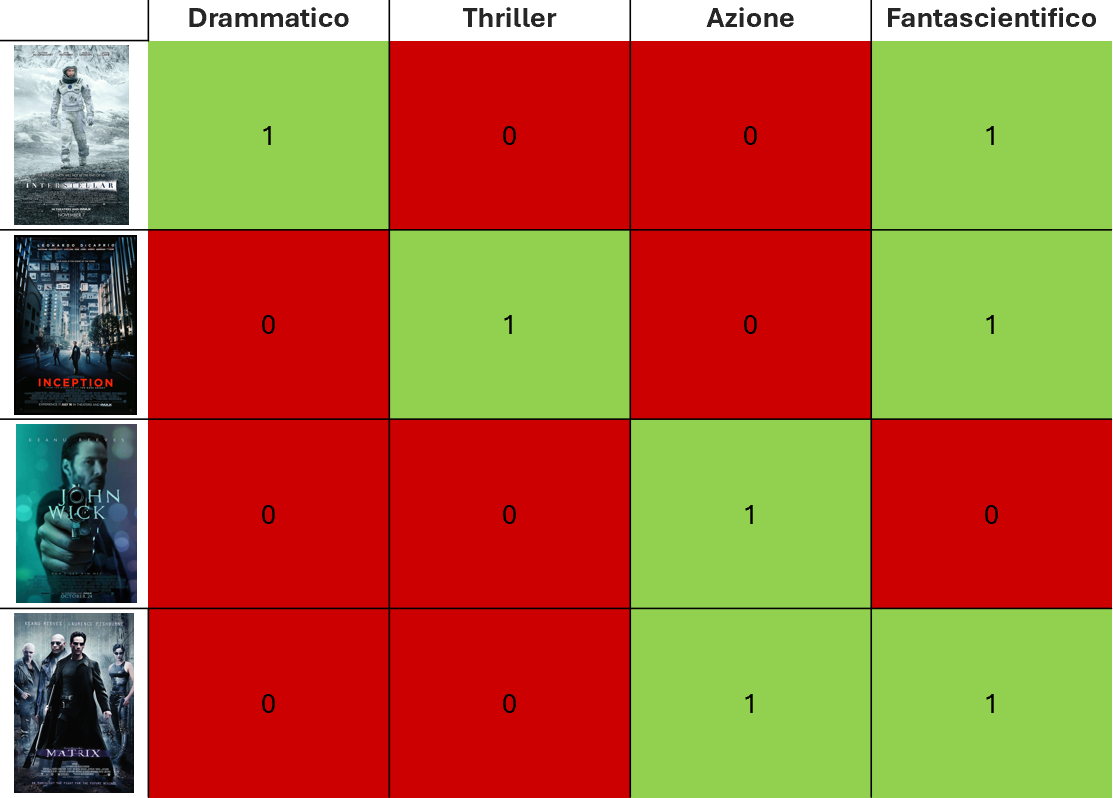
\includegraphics[scale=0.5]{figures/content_based_filtering.PNG}
    \caption{La figura mostra i vettori delle caratteristiche dei film (in questo caso il genere) per i film in esempio. Se il film appartiene ad uno specifico genere viene posto il valore $1$, altrimenti $0$}
    \label{fig:item_vector}
\end{figure}

Si creano vettori per i film considerando tutti i generi analizzati fino ad ora e si calcola la similarità con il profilo dell'utente. Si ottiene, utilizzando per esempio la similarità coseno, un valore di $0.47$ per $Interstellar$ e di $0.67$ per \textit{John Wick}, quindi quest'ultimo viene raccomandato prima di \textit{Interstellar}, perché è più simile al profilo dell'utente.

\subsubsection{Vantaggi e svantaggi}

I vantaggi di quest'approccio sono:
\begin{itemize}
    \item il modello non ha bisogno di dati su altri utenti, poiché le raccomandazioni sono specifiche per questo utente. Questo lo rende più facile da scalare a un grande numero di utenti
    \item il modello può catturare gli interessi specifici di un utente e può raccomandare \textit{item} di nicchia che interessano a pochissimi altri utenti
\end{itemize}

Gli svantaggi di quest'approccio sono:
\begin{itemize}
    \item poiché la rappresentazione delle caratteristiche degli oggetti è in parte progettata manualmente, questa tecnica richiede molta conoscenza del dominio. Il modello può essere solo quindi valido quanto le caratteristiche progettate manualmente
    \item il modello può fare raccomandazioni solo basate sugli interessi esistenti dell'utente. In altre parole, ha una capacità limitata di espandere gli interessi dell'utente
\end{itemize}

\subsection{Collaborative filtering}
Il \textit{collaborative filtering} (\textit{CF}) viene introdotto per la prima volta dal sistema \textit{Tapestry}~\cite{Tapestry} e si riferiva al fatto che \textit{"people collaborate to help one another perform the filtering process in order to handle the large amounts of email and messages posted to newsgroups"}. Questo termine ha poi assunto significati più ampi. In senso generale, indica il processo di filtraggio di informazioni o pattern tramite tecniche che coinvolgono la collaborazione tra più utenti, agenti e fonti di dati. Il \textit{CF} esiste in molte forme e, sin dalla sua introduzione, sono stati proposti numerosi metodi basati su di esso. Per affrontare alcune delle limitazioni del \textit{content-base filtering}, il \textit{collaborative filtering} utilizza simultaneamente le somiglianze tra utenti e \textit{item} per fornire raccomandazioni. I modelli possono raccomandare un \textit{item} all'utente $A$ in base agli interessi di un utente simile $B$ anche se $A$ non ha mai visto \textit{item} simili. In generale, le tecniche di \textit{CF} possono essere suddivise in tre categorie: \textit{CF} basato sulla memoria, \textit{CF} basato su modelli e i modelli ibridi~\cite{Su}. Tra le tecniche rappresentative basate sulla memoria ci sono i metodi \textit{nearest neighbor-based}, come il \textit{CF} basato sugli utenti (\textit{user-based}) e quello basato sugli oggetti (\textit{item-based})~\cite{Sarwar}. I modelli a fattori latenti, come la \textit{Matrix Factorization}, sono esempi di \textit{CF} basato su modelli. Il \textit{CF} basato sulla memoria presenta delle limitazioni nella gestione di dati sparsi e su larga scala, poiché calcola la similarità basandosi sugli oggetti in comune. I metodi basati su modelli sono diventati più popolari grazie alla loro maggiore efficacia nel gestire la sparsità e la scalabilità. Molti approcci \textit{CF} basati su modelli possono essere estesi con reti neurali, permettendo modelli più flessibili e scalabili grazie all'accelerazione computazionale offerta dal \textit{Deep Learning}~\cite{Zhang}. In generale, il \textit{CF} utilizza i dati di interazione tra utenti e oggetti per fare previsioni e raccomandazioni.


\subsubsection{Esempio}

Si supponga di avere una matrice di interazioni tra utenti e \textit{item}, in cui ogni riga corrisponde ad un utente e ogni colonna corrisponde ad un \textit{item}. Ogni elemento della matrice rappresenta il feedback dell'utente sull'\textit{item}, ad esempio una valutazione numerica o un'indicazione binaria di interesse.

L'idea principale del modello è la seguente:

\begin{itemize}
    \item calcolare la similarità tra gli utenti (o alternativamente tra gli \textit{item}) utilizzando la similarità coseno
    \item utilizzare queste similarità per prevedere il grado di interesse di un utente verso un \textit{item} non ancora valutato, basandosi sui voti dati da utenti simili
\end{itemize}

La similarità coseno tra due vettori \( \mathbf{x}, \mathbf{y} \in \mathbb{R}^n \) è definita come:

\[
\text{sim}(\mathbf{x}, \mathbf{y}) = \cos(\theta) = \frac{\mathbf{x} \cdot \mathbf{y}}{\|\mathbf{x}\|_2 \|\mathbf{y}\|_2}
\]

Nel contesto del modello, ad esempio, i vettori \( \mathbf{x} \) e \( \mathbf{y} \) rappresentano le rispettive righe della matrice di interazione, ossia le valutazioni degli utenti sui diversi film. Per prevedere la valutazione che l'utente potrebbe dare ad un film si considera la media delle valutazioni date dagli utenti al film pesata dalla similarità tra l'utente iniziale e gli altri.

Si supponga di voler raccomandare un film all'utente \textit{Verde}, in particolare prevedere il punteggio che potrebbe assegnare al film \textit{Fight Club}, che non ha ancora visto.

\begin{figure}[htbp]
    \centering
    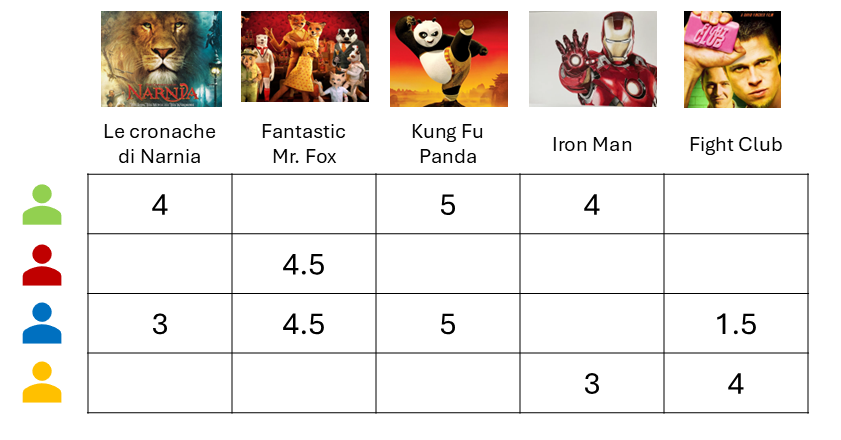
\includegraphics[scale=0.5]{figures/collaborative_filtering/interaction_matrix.png}
    \caption{matrice di interazione tra utenti e film. Le righe rappresentano gli utenti, le colonne i film e gli elementi della matrice i voti che l'utente ha dato al film. Se l'utente non ha visto il film, l'elemento della matrice è vuoto.}
\end{figure}

Si calcola la similarità coseno tra l'utente \textit{Verde} e gli altri utenti che hanno visto il film. 

Similarità tra Verde e Blu:

\[
\text{sim}(Verde, Blu) = \frac{4 \cdot 3 + 0 \cdot 4.5 + 5 \cdot 5 + 4 \cdot 0 + 0 \cdot 1.5}{\sqrt{4^2 + 0 + 5^2 + 4^2 + 0} \cdot \sqrt{3^2 + 4.5^2 + 5^2 + 0 + 1.5^2}} \approx 0.65
\]

Similarità tra Verde e Giallo:

\[
\text{sim}(Verde, Giallo) = \frac{4 \cdot 0 + 0 \cdot 0 + 5 \cdot 0 + 4 \cdot 3 + 0 \cdot 4}{\sqrt{57} \cdot \sqrt{0 + 0 + 0 + 9 + 16}} \approx 0.319
\]

Ora, la predizione per l'utente \textit{Verde} per \textit{Fight Club} si calcola come media pesata:

\[
\frac{0.65 \times 1.5 + 0.32 \times 4}{0.65 + 0.32} \approx 2.33
\]

Quindi si prevede che l'utente verde valuterebbe il film \textit{Fight Club} con un voto intorno a 2.33.

Il modello basato sulla similarità coseno è semplice da implementare e intuitivo, ma può soffrire di problemi come la scarsità di dati e l'effetto del rumore nelle valutazioni. Tuttavia, rimane un punto di partenza valido per sistemi di raccomandazione collaborativi. Se si considerassero solamente i contribuiti dei $k$ utenti più simili, si potrebbe migliorare la robustezza della previsione. Questo approccio è noto come \textit{K-Nearest Neighbors} (\textit{KNN}).

\subsubsection{Vantaggi e svantaggi}

I vantaggi di quest'approccio sono:

\begin{itemize}
  \item non è necessaria conoscenza del dominio: nel \textit{CF}, la raccomandazione si basa esclusivamente sulle valutazioni o interazioni passate degli utenti con gli \textit{item}, senza utilizzare informazioni aggiuntive sulle caratteristiche degli stessi. Questo significa che il modello non richiede conoscenza specifica del dominio (ad esempio il genere di un film o le preferenze dettagliate degli utenti), ma si limita a individuare pattern di comportamento simili tra utenti o \textit{item}. Di conseguenza, il sistema è applicabile in diversi contesti in modo generale e automatico, apprendendo le affinità direttamente dai dati di interazione.
  \item serendipità: anche se il modello non sa che l'utente è interessato a un determinato \textit{item} potrebbe comunque raccomandarlo perché utenti simili sono interessati a quell'\textit{item}

\end{itemize}

Gli svantaggi di quest'approccio sono:

\begin{itemize}
  \item non si può gestire \textit{item} nuovi: il \textit{CF} classico fatica a gestire \textit{item} nuovi, cioè quelli che non hanno ancora ricevuto valutazioni o interazioni dagli utenti (problema del \textit{cold start}). Senza dati storici il modello non può calcolare similarità né fare previsioni attendibili
  \item difficoltà nell'includere caratteristiche aggiuntive per \textit{query}/\textit{item}: le caratteristiche aggiuntive (\textit{side features}) sono tutte quelle informazioni oltre all'id dello user o dell'\text{item}. Per esempio, per i film, le caratteristiche possono includere il paese o l'età. Includere queste caratteristiche migliora la qualità del modello
\end{itemize}

\subsubsection{Approcci}

Esistono due approcci principali per facilitare tale confronto, che costituiscono le due tecniche fondamentali del \textit{collaborative filtering}: 

\begin{itemize}
    \item approcci \textit{neighborhood}: si concentrano sulle relazioni tra \textit{item} oppure, alternativamente, tra utenti. Un approccio \textit{item}-\textit{item} modella la preferenza di un utente per un \textit{item} sulla base delle valutazioni di \textit{item} simili da parte dello stesso utente
    \item modelli basati sulla \textit{Matrix Factorization}: un approccio in cui sia gli \textit{item} che gli utenti vengono proiettati in uno stesso spazio latente, cercando di spiegare le valutazioni osservate attraverso fattori latenti inferiti automaticamente dai feedback
\end{itemize}

\section{Matrix Factorization}\label{matrix_factorization}

La \textit{Matrix Factorization} è una tecnica utilizzata per rappresentare una matrice come prodotto di due o più matrici. Consente di estrarre automaticamente strutture latenti dai dati, rendendo possibile la scoperta di relazioni implicite tra entità \cite{MC}. Questa tecnica è alla base di molte applicazioni in ambiti diversi, tra cui l'elaborazione di segnali, la compressione dei dati, la visione artificiale e, in particolare, i sistemi di \textit{recommendation}.

Formalmente, data una matrice $R \in \mathbb{R}^{m \times n}$, la fattorizzazione mira a trovare due matrici $W \in \mathbb{R}^{m \times k}$ e $H \in \mathbb{R}^{n \times k}$ tali che:
\[
R \approx WH^T
\]
dove 
\begin{itemize}
    \item le righe di $W$ corrispondono agli \textit{embedding} degli utenti
    \item le righe di $H$ corrispondono agli \textit{embedding} degli \textit{item}
    \item $k \ll \min(m,n)$ è il rango latente scelto
\end{itemize}

\begin{figure}[htbp]
    \centering
    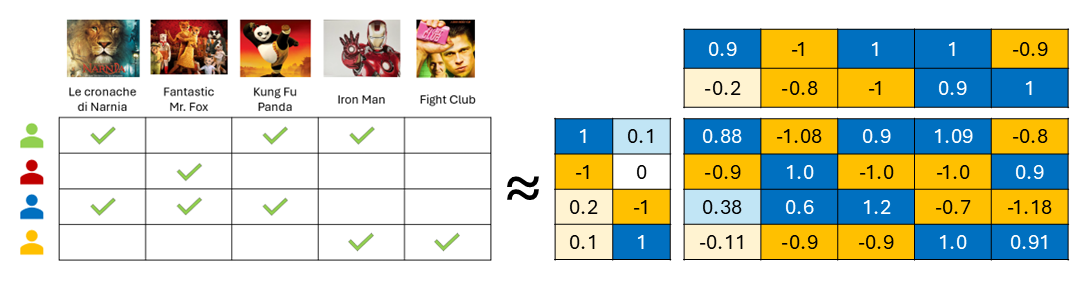
\includegraphics[scale=0.5]{figures/collaborative_filtering/matrix_factorization.PNG}
    \caption{rappresentazione della matrice $R$ come prodotto delle due matrici $W$ e $H$}
    \label{fig:matrix_factorization}
\end{figure}

Questa approssimazione riduce la dimensionalità dei dati, semplifica il modello e cattura le relazioni principali presenti nella matrice originaria. Un celebre esempio dell'efficacia di questa tecnica nei sistemi di \textit{recommendation} è il \textit{Netflix Prize} del 2006. Il team vincente la utilizzò per migliorare le previsioni di rating del 10\% rispetto al sistema originario di Netflix \cite{TheNP}. I principali vantaggi nel suo utilizzo sono la scalabilità, poiché i modelli sono efficienti da memorizzare e computare, e la capacità di generalizzazione, in quanto riescono a catturare relazioni latenti non esplicitamente osservate. Tuttavia, esistono anche alcuni limiti, tra cui il problema della \textit{cold start}, che rende difficile raccomandare per nuovi utenti o nuovi \textit{item}, e la sparsità, che può portare a una una bassa qualità delle raccomandazioni\cite{SVD_analysis}. Pur con alcune limitazioni, essa costituisce la base per molti degli algoritmi di \textit{recommendation} più efficaci oggi in uso, ed è spesso integrata con approcci più complessi, come i modelli \textit{Deep Learning} o i grafi.

\subsection{Concetto di Spazio Latente ed Embedding}
Nel contesto della \textit{Matrix Factorization}, uno dei concetti centrali è lo spazio latente. Questo spazio rappresenta un insieme di dimensioni astratte, non osservabili direttamente, ma che spiegano le correlazioni nei dati. Ad esempio, in un sistema di raccomandazione di film, utenti e film possono essere rappresentati come vettori in uno spazio $k$-dimensionale, dove ogni dimensione può rappresentare una caratteristica latente come la preferenza per il genere "azione", la complessità della trama, il livello di drammaticità, ecc. Queste dimensioni non sono etichettate esplicitamente, ma vengono apprese automaticamente durante l'addestramento. Questa rappresentazione vettoriale in uno spazio latente prende il nome di \textit{embedding}. Ogni utente e ogni \textit{item} (ad esempio, film, prodotto o articolo) viene associato a un vettore numerico che cattura le sue proprietà implicite in modo compatto.

\subsection{Apprendimento delle Feature}
Le feature apprese nel contesto della matrix factorization non sono predefinite, ma emergono come risultato dell'ottimizzazione. In pratica, si cerca di minimizzare una funzione di perdita, tipicamente la somma dei quadrati degli errori tra le valutazioni osservate e quelle predette:

\[
\min_{U,V} \sum_{(i,j) \in \mathcal{K}} (R_{ij} - W_i \cdot H_j^T)^2 + \lambda ( \|W_i\|^2 + \|H_j\|^2 )
\]

dove:
\begin{itemize}
    \item $\mathcal{K}$ è l'insieme delle coppie $(i,j)$ per cui $R_{ij}$ è noto;
    \item $\lambda$ è un termine di regolarizzazione che evita l'overfitting.
\end{itemize}

Durante l'ottimizzazione, i vettori $W_i$ e $H_j$ vengono aggiornati in modo tale da minimizzare l'errore sulle osservazioni note, catturando implicitamente le caratteristiche principali che influenzano le preferenze. I modelli apprendono automaticamente un vettore di \textit{embedding} per ciascun utente che spieghi al meglio le sue preferenze. Di conseguenza, gli \textit{embedding} di utenti con gusti simili risulteranno vicini tra loro. Allo stesso modo il modello apprende gli \textit{embedding} dei 
\textit{item} in modo da spiegare al meglio la matrice di feedback

\subsection{Esempio}

Per esempio si consideri un sistema di \textit{recommendation} di film in cui i dati di addestramento consistono in una matrice di feedback in cui:

\begin{itemize}
    \item Ogni riga rappresenta un utente
    \item Ogni colonna rappresenta un \textit{item} (un film)
    \item Il feedback sui film rientra in una delle due categorie:
    \begin{itemize}
        \item esplicito: gli utenti specificano quanto gli è piaciuto un determinato film fornendo una valutazione numerica
        \item implicito: se un utente guarda un film, il sistema deduce che l'utente è interessato
    \end{itemize}
\end{itemize}

Per semplificare, si supponga che la matrice di feedback sia binaria; cioè il simbolo "check" verde indica interesse per il film.

Quando un utente visita la homepage, il sistema dovrebbe raccomandare film basati su:

\begin{enumerate}
    \item somiglianza con i film che l'utente ha apprezzato in passato
    \item film che utenti simili hanno apprezzato
\end{enumerate}

Il modello, applicando la tecnica di \textit{Matrix Factorization} ottiene in maniera automatica una rappresentazione degli utenti e dei film in uno spazio di \textit{embedding} a bassa dimensione. In questo spazio, gli utenti e i film sono rappresentati da vettori che catturano le loro caratteristiche latenti. Per esempio il modello potrebbe apprendere due dimensioni latenti per i film: la prima esprime se il film è per adulti o per bambini mentre la seconda esprime il grado in cui il film è un \textit{blockbuster} (film molto popolare e di grande successo al botteghino) o un film d'autore. Stessa cosa succede per gli utenti: il modello apprende le preferenze degli utenti in relazione a queste due dimensioni latenti. Si può pensare allo spazio di \textit{embedding} come a una rappresentazione astratta comune sia agli \textit{item} che agli utenti.

\begin{figure}[htbp]
    \centering
    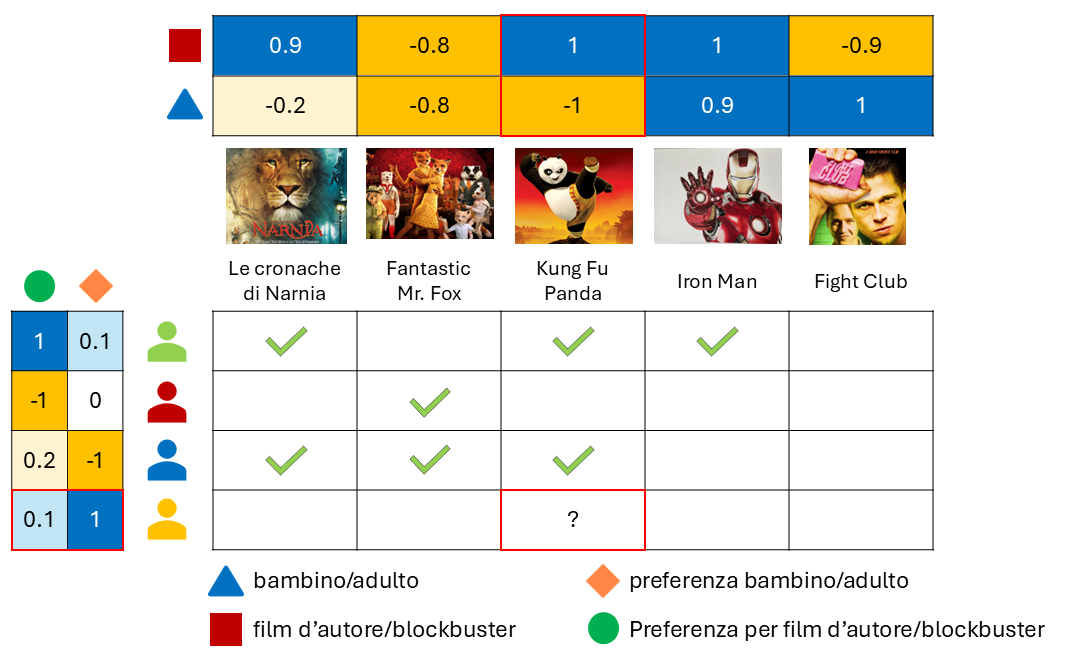
\includegraphics[scale=0.4]{figures/collaborative_filtering/2D_matrix.PNG}
    \caption{matrice che mostra i film guardati dagli utenti, le categorie dei film e le preferenze degli utenti estese}
    \label{fig:2D_matrix}
\end{figure}


La previsione del gradimento di un utente per un film si ottiene calcolando il prodotto scalare tra l'embedding dell'utente e quello del film.

\[
r_{ui} = w_u \cdot h_i
\]

Se si volesse calcolare il gradimento dell'utente \textit{Giallo} per il film \textit{Kung Fu Panda}, si calcolerebbe il prodotto scalare tra i rispettivi \textit{embedding}:

\[
\begin{bmatrix}
0.1 & 1
\end{bmatrix}
\times
\begin{bmatrix}
1 \\
-1
\end{bmatrix} = -0.9
\]

quindi il modello prevede che l'utente \textit{Giallo} non apprezzi il film \textit{Kung Fu Panda}.

\subsection{Vantaggi e svantaggi}
I vantaggi della \textit{Matrix Factorization} includono:
\begin{itemize}
    \item scalabilità: la \textit{Matrix Factorization} può gestire matrici molto grandi e sparse, tipiche dei sistemi reali
    \item generalizzazione: le feature apprese permettono di effettuare predizioni su dati mai visti prima (\textit{cold-start}), anche se con alcune limitazioni
    \item compattezza: gli \textit{embedding} permettono una rappresentazione compatta ma espressiva delle entità
\end{itemize}

Gli svantaggi della \textit{Matrix Factorization} includono:

\begin{itemize}
    \item ottimizzazione complessa: l'addestramento può essere computazionalmente costoso e sensibile all'inizializzazione e ai parametri di regolarizzazione
    \item scarsa interpretabilità: gli \textit{embedding} latenti non sono facilmente interpretabili, rendendo difficile spiegare le raccomandazioni agli utenti
\end{itemize}